\documentclass{beamer}

% Theme choice
\usetheme{CambridgeUS} % professional, clean look
\usecolortheme{default} % colors can be adjusted if desired

% Packages
\usepackage[utf8]{inputenc}
\usepackage{graphicx}   % for including graphics
\usepackage{booktabs}   % for tables
\usepackage{amsmath, amssymb} % for math
\usepackage{hyperref}   % for clickable links

% Title page info
\title{Comfort or Cost? Wages vs Amenities in Migration Decisions Later in Life}
\author[Tate Mason]{Tate Mason \\ \smallskip \texttt{Tate.Mason@uga.edu}}
\institute[Univ. of Georgia]{John Munro Godfrey Sr. Department of Economics \\ The University of Georgia}
\date{\today} % or custom date

% Begin document
\begin{document}

% Title page
\begin{frame}
  \titlepage
\end{frame}

% Outline
\begin{frame}{Outline}
  \tableofcontents
\end{frame}

\section{Introduction}
\begin{frame}{Motivation}
  \begin{itemize}
    \item Typically, location choice models focus on wages.
    \item Do other factors play a role in location decisions later in life?
    \item \textbf{Main Question:} How does motivation for moving change with age?
  \end{itemize}
\end{frame}

\section{Data}
\begin{frame}{Data Source}
  \begin{itemize}
    \item IPUMS USA data from 1990 - 2019
    \item Decennial censuses and ACS data
    \item CMS data for health care costs
    \item DOE data for average climate conditions
    \item Panel structure by linking individuals across years
  \end{itemize}
\end{frame}

\begin{frame}{Sample Selection}
  \begin{itemize}
    \item Individuals aged 40-80
    \item Moved at least once during observation period
    \item Exclude group quarters, military, and missing data
    \item Final sample size: ~1.25 million households
  \end{itemize}
\end{frame}

\section{Empirical Facts}
\begin{frame}{Empirical Motivation}
  \begin{itemize}
    \item Younger movers and older movers exhibit different mobility patterns
    \item High income individuals move more with higher frequency
    \item Those without children move more often
    \item Probability of moving peaks at the age around retirement, and then declines
  \end{itemize}
\end{frame}

\begin{frame}{Summary Statistics}
  \begin{table}[htbp]
  \centering
  \caption{Summary Statistics}
  \label{tab:summ_stats}
    \begin{tabular}{|l|c|}
      \hline
       & Mean \\
      \hline
      n & 21,138,046 \\
      Age & 57.62 \\
      Wages & 33251.83 \\
      Gross Rent & 170.07\\
      Health Costs & 6336.11 \\
      Mover \% & 17\% \\
      \hline
    \end{tabular}
  \end{table}
\end{frame}

\begin{frame}{Graphical Evidence}
  \begin{figure}
    \centering
    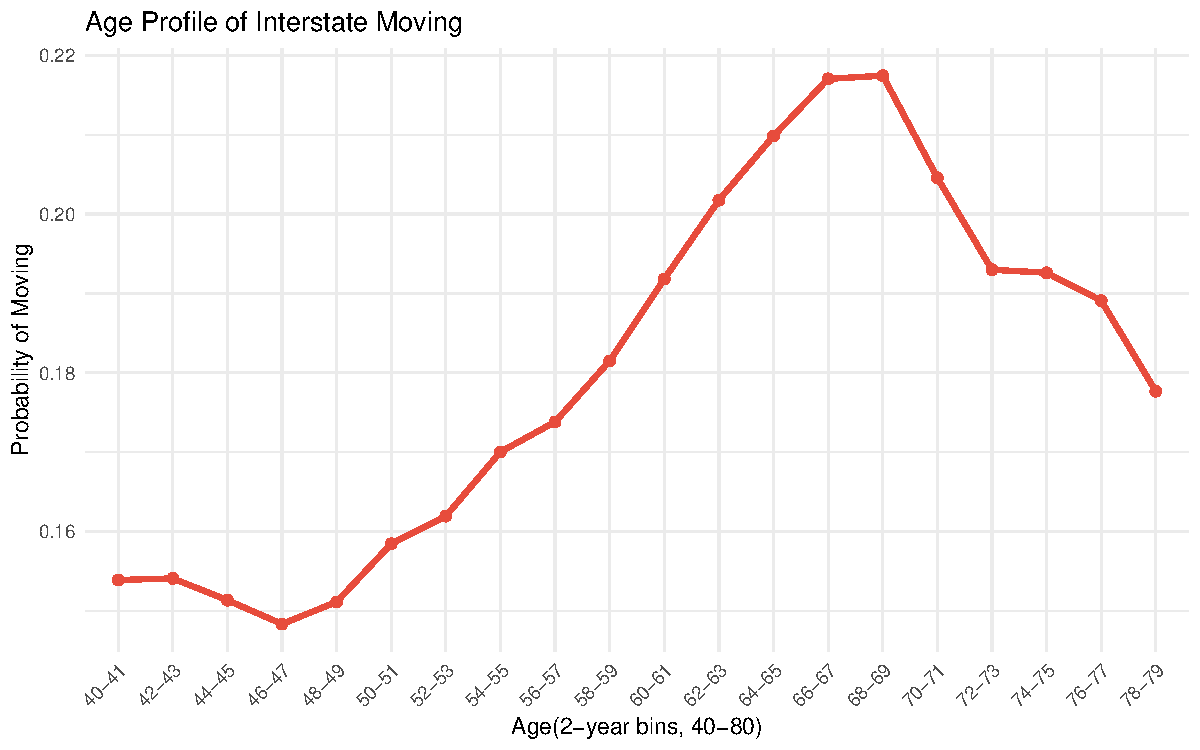
\includegraphics[width=0.8\linewidth]{figures/age_profile_move.pdf}
    \caption{Age Profile of Moving Frequency}
  \end{figure}
\end{frame}
\begin{frame}{Graphical Evidence}
  \begin{figure}
    \centering
    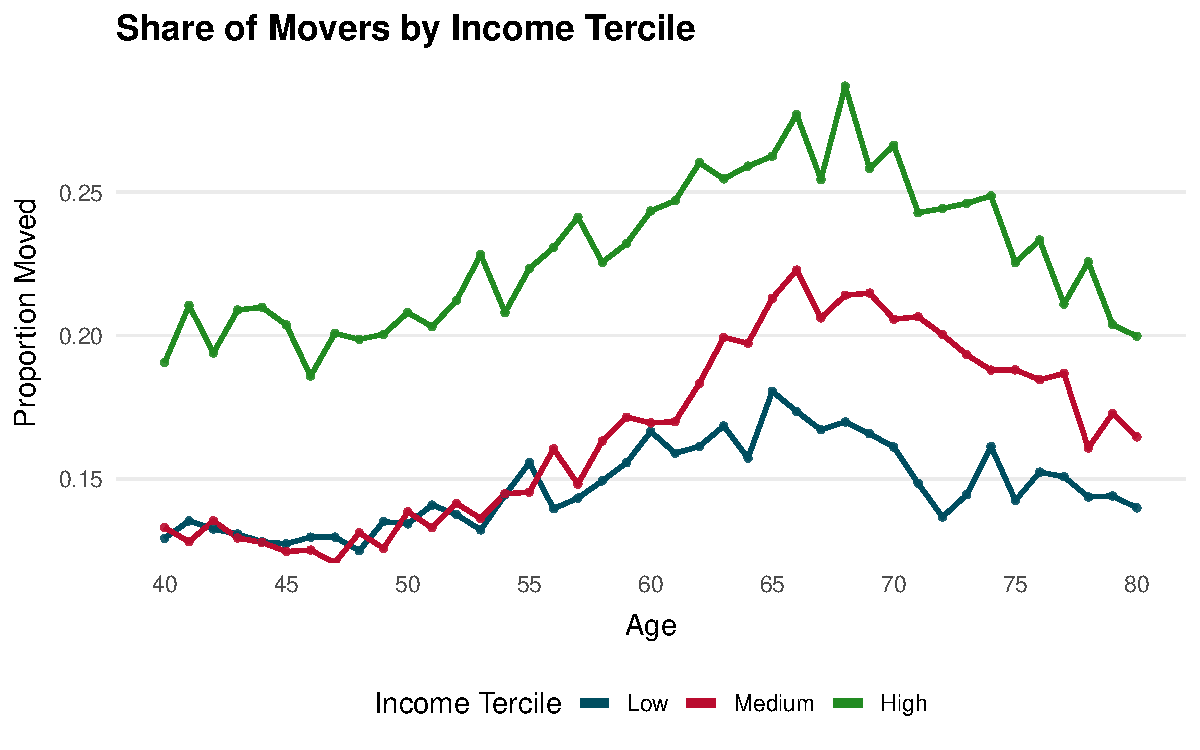
\includegraphics[width=0.8\linewidth]{figures/mover_prop_income.pdf}
    \caption{Income vs Moving Frequency}
  \end{figure}
\end{frame}
\begin{frame}{Graphical Evidence}
  \begin{figure}
    \centering
    
\includegraphics[width=0.8\linewidth]{~/SchoolWork/Y2S1/Macro/ResearchCalibration/Figs/top10_flows.pdf}
    \caption{Top 10 Migration Flows}
  \end{figure}
\end{frame}
\section{Model}
\begin{frame}{Model Overview}
  \begin{itemize}
    \item Two types: Workers, Retirees
    \item Both types maximize lifetime utility over consumption and amenities
    \item Hold prior beliefs $\delta$ about all $z'\ne z$ which are discarded upon moving, and new beliefs are formed
  \end{itemize}
\end{frame}
\begin{frame}{Utility Function}
  \begin{itemize}
    \item Workers: $U^w(c, ;t) = \frac{(c-\bar{c})^(1-\sigma)}{1-\sigma} - \gamma\cdot\{z'\ne z\}$
    \item Retirees: $U^r(c, m(z);t) = \frac{(c-\bar{c})^(1-\sigma)}{1-\sigma} + m(z) - \gamma\cdot\{z'\ne z\}$
    \item $c$: consumption, $m(z)$: amenities in location $z$
    \item $\gamma$: moving cost parameter
  \end{itemize}
\end{frame}
\begin{frame}{Budget Constraints}
  \begin{itemize}
    \item Workers: $c = w(z) - \tau(z) - \mathbb{E}[c(h(z))|\delta]$
    \item $\delta$: Prior assumptions about housing costs in location $z'$
    \item $w(z)$: wage in location $z$, $\tau(z)$: taxes, $c(h(z))$: housing cost (rent)
    \item Retirees: $c_t = p(1-\tau(z))w(z) - \mathbb{E}[c(hc(z))|\delta]$
    \item $p$: pension replacement rate, $hc(z)$: health care cost 
  \end{itemize}
\end{frame}
\begin{frame}{Decision Problem: Workers}
  \begin{equation}
    $V^w(\delta, z, t) = \max\{V_w^M(\delta, z, t), V_w^S(\delta, z, t)\}$
  \end{equation}
  \begin{itemize}
    \item $V_w^M$: value of moving, $V_w^S$: value of staying
  \end{itemize}
  \begin{equation}
    \item $V^S_w(\delta, z; t) = \max_{c} \{U(c) + V^w(\delta, z_t, t+1)\}$
  \end{equation}
  \begin{equation}
    \item $V^M_w(\delta, z; t) = \max_{z', c} \{U(c) + \beta\mathbb{E}[V^w(\delta', z'; t+1)|\delta]|\delta])\}$
  \end{equation}
\end{frame}
\begin{frame}{Decision Problem, Retirees}
  \begin{equation}
    $V^r(\delta, z; t) = \max\{V_r^M(\delta, z; t), V_r^S(z; t)\}$
  \end{equation}
  \begin{itemize}
    \item $V_r^M$: value of moving, $V_r^S$: value of staying
  \end{itemize}
  \begin{equation}
    \item $V^S_r(z; t) = \max_{c} \{U(c, m(z)) + \beta V^r(\delta, z; t+1)\}$
  \end{equation}
  \begin{equation}
    \item $V^M_r(\delta, z; t) = \max_{z', c} \{U(c, m(z')) + \beta V^r(\delta', z'; t+1)\}$
  \end{equation}
\end{frame}
\section{Estimation and Results}
\begin{frame}{Estimation Strategy}
  \begin{itemize}
    \item Use method of simulated moments (MSM)
    \item Set parameters: prior belief parameters $\delta$, utility curvature $\sigma$, discount factor $\beta$
    \begin{itemize}
      \item $\beta = 0.96$ fixed
      \item $\sigma = 2$ fixed
      \item $\delta = [-1, 0, 1]$
    \end{itemize}
    \item Recover moving cost parameter $\gamma$ for each group
    \begin{itemize}
      \item Workers: $\gamma_w = 6.37$
      \item Retirees: $\gamma_r = 4.75$
    \end{itemize}
    \item Simulated moments: age-specific moving rates and migration flow patterns
  \end{itemize}
\end{frame}
\begin{frame}{Graphical Results}
  \begin{figure}
    \centering
    
\includegraphics[width=0.8\linewidth]{~/SchoolWork/Y2S1/Macro/ResearchCalibration/Figs/age_profiles_model_vs_data.pdf}
    \caption{Age Profile of Moving Frequency: Model vs Data}
  \end{figure}
\end{frame}
\begin{frame}{Graphical Results}
  \begin{figure}
    \centering
    
\includegraphics[width=0.8\linewidth]{~/SchoolWork/Y2S1/Macro/ResearchCalibration/Figs/top10_flows.pdf}
    \caption{Migration Flows: Data}
  \end{figure}
\end{frame}
\begin{frame}{Graphical Results}
  \begin{figure}
    \centering
    
\includegraphics[width=0.8\linewidth]{~/SchoolWork/Y2S1/Macro/ResearchCalibration/Figs/top10_model_flows.pdf}
    \caption{Migration Flows: Model}
  \end{figure}
\end{frame}
\begin{frame}{Discussion}
  \begin{itemize}
    \item Model captures general trajectory of moving rates with age, with exception of oldest group
    \item Model fails to capture migration flow patterns for both groups
    \item Clearly more work to do on this front, suggestions welcome!
  \end{itemize}
\end{frame}
\begin{frame}{Thank You}
  \begin{center}
    \Huge Thank You! \\
    \vspace{1cm}
    \Large Questions?
  \end{center}
\end{frame}

\end{document}
